% ─── Figure 1 ────────────────────────────────────────────────────────────────
% Assembled 6-panel main result figure (Inkscape).
% Individual source panels: outputs/main/fig2a–fig4b.
% Experimental design figure → Supplementary Fig. S1 (figures/sup1.png).
%
% Cross-reference note: labels previously on separate figures are now unified:
%   \label{fig:main}  replaces  fig:bout_main / fig:washout / fig:tf_cluster

\begin{figure}[!h]
\centering
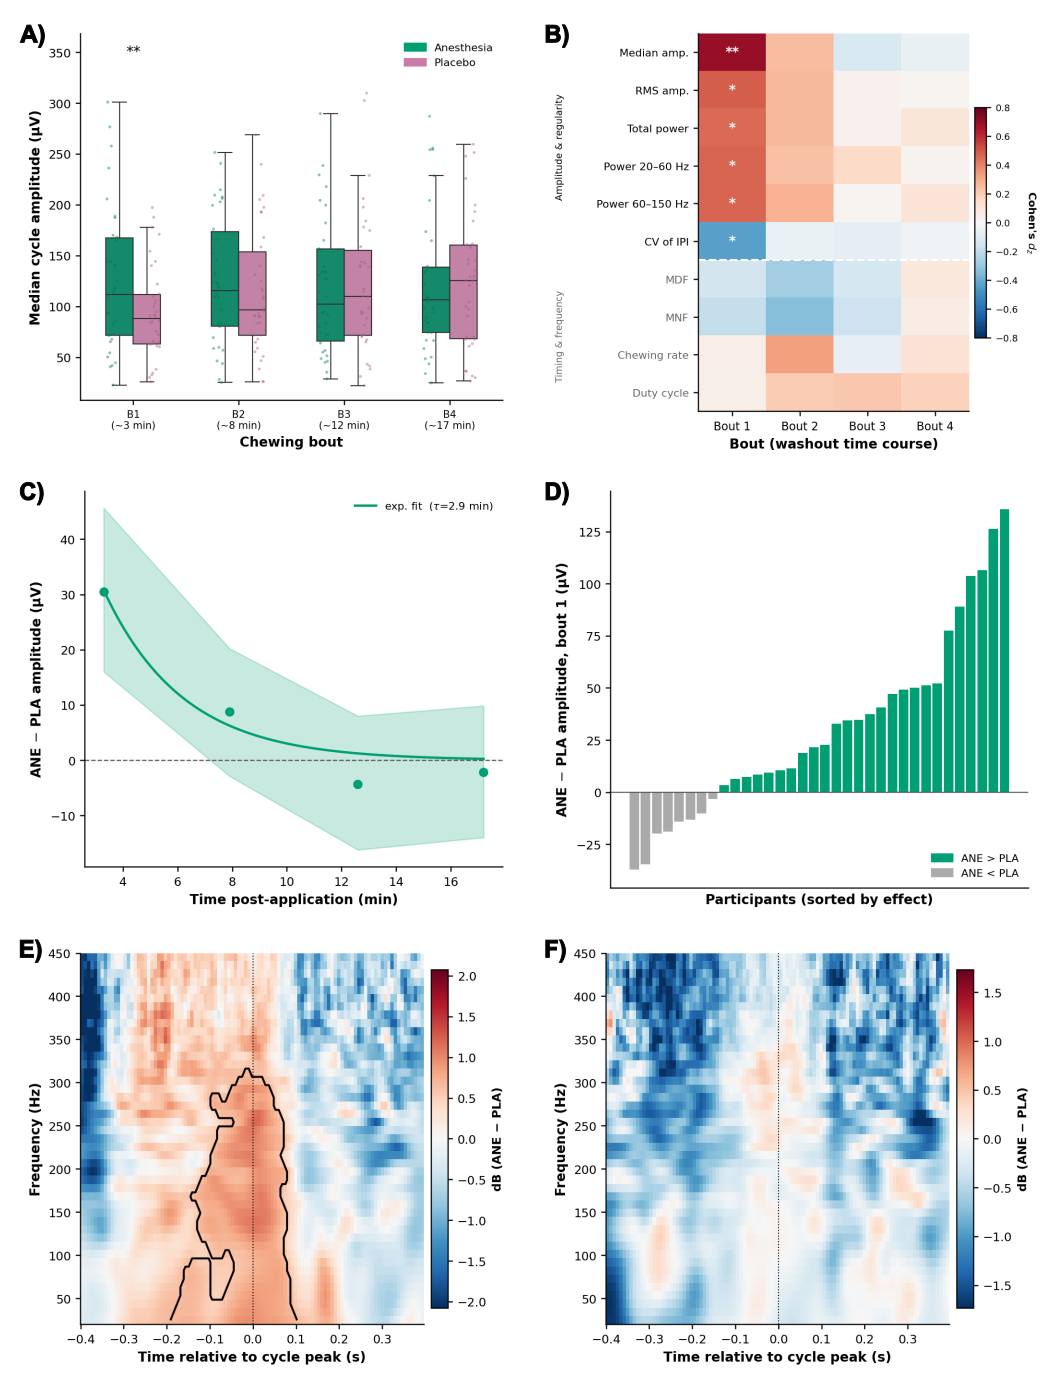
\includegraphics[width=\linewidth]{figures/fig1.png}
\caption{\textbf{Transient sensorimotor gain compensation under masticatory
anesthesia ($N$\,=\,34).}
\textbf{(A)} Median cycle amplitude (\textmu{}V) and \textbf{(B)} coefficient
of variation of the inter-peak interval (CV\textsubscript{IPI}) for
anesthesia (green) and placebo (lilac) across chewing bouts~1--4.
Boxes show median and interquartile range; individual participants overlaid as
jittered points.
Effect size ($d_z$) and FDR-corrected significance are labelled above bout~1
(**: $p_{\text{FDR}}$\,<\,0.01; *: $p_{\text{FDR}}$\,<\,0.05;
Benjamini--Hochberg~\cite{Benjamini1995} across 11~metrics).
\textbf{(C)} Effect-size heatmap ($d_z$, ANE\,$-$\,PLA) for all EMG metrics
(rows) and bouts~1--4 (columns).
White asterisks mark cells surviving FDR correction at bout~1
($p_{\text{FDR}}$\,<\,0.05).
Amplitude and regularity metrics (upper block, black labels) show a transient
gain at bout~1 that converges to zero by bouts~3--4; timing and frequency
metrics (lower block, grey labels) show no effect at any bout.
\textbf{(D)} ANE\,$-$\,PLA difference in median cycle amplitude across bouts
($\approx$\,3, 7.5, 12, and 17~min post-application; error bars: 95\%
bootstrap CI).
Solid curve: exponential decay fit ($\tau$\,$\approx$\,2.9~min), consistent
with topical lidocaine pharmacokinetics~\cite{vonGunten2019}.
\textbf{(E)} Amplitude difference at bout~1 per participant, sorted by
magnitude; green bars: ANE\,$>$\,PLA; grey bars: ANE\,$<$\,PLA.
76\% of participants (26/34) showed greater amplitude under anesthesia
(Wilcoxon $p$\,=\,0.0003).
\textbf{(F)} Grand-average anesthesia-minus-placebo Morlet scalograms
(20--450~Hz; $x$-axis: time relative to cycle peak) at bout~1 (top) and
bout~4 (bottom).
Black contour: significant cluster at bout~1 (cluster-based permutation
test~\cite{Maris2007}; $p$\,=\,0.036; $\approx$\,30--300~Hz,
$-$0.15 to $+$0.1~s relative to cycle peak).
No significant cluster at bout~4 ($p_{\min}$\,=\,0.59).}
\label{fig:main}
\end{figure}
